\documentclass[apectratio=43,unicode]{beamer}
\usetheme{Moscow}

\usepackage[utf8]{inputenc}
\usepackage[T2A]{fontenc}
\usepackage[main=russian,english]{babel}

\usepackage{amsmath,amssymb}

\renewcommand{\thefootnote}{\fnsymbol{footnote}}
\hypersetup{
	pdfauthor={Ivan Tsybulin}
}

\usepackage{euler}
\usepackage{mathtools}

\graphicspath{{images//}}

\title[СЛАУ]{Системы линейных алгебраических уравнений\\Часть 1. Матричные нормы. Обусловленность}
\author[Цыбулин И.В.]{Скалько Юрий Иванович\\
\textbf{Цыбулин Иван}}
\date{}

\newcommand{\colorhref}[2]{\href{#1}{\textcolor{miptbase!30!black}{#2}}}

\begin{document}

\begin{frame}[plain]
\titlepage
\end{frame}

\newcommand\myframe[2]{\subsection{#1}\frame{\frametitle{#1}{#2}}}

\section{ }

\newcommand{\A}{{\mathbf{A}}}
\newcommand{\x}{{\mathbf{x}}}
\newcommand{\y}{{\mathbf{y}}}
\renewcommand{\b}{{\mathbf{b}}}

\newcommand{\one}{{\ell_1}}
\newcommand{\tr}{{\mathsf{T}}}

\section{СЛАУ}

\subsection{Задача СЛАУ}
\begin{frame}
\frametitle{Постановка задачи}
	Дана квадратная матрица $\A$ 	и столбец $\b$
	$$
	\A =
	\begin{pmatrix}
	a_{11}&a_{12}&\dots&a_{1n}\\
	a_{21}&a_{22}&\dots&a_{2n}\\
	\vdots&\vdots&\ddots&\vdots\\
	a_{n1}&a_{n2}&\dots&a_{nn}\\
	\end{pmatrix}
	,\quad
	\b =
	\begin{pmatrix}
	b_{1}\\
	b_{2}\\
	\vdots\\
	b_{n}\\
	\end{pmatrix}
	,\quad \det \A \neq 0
	$$

	Решить систему линейных алгебраических уравнений 
	$$
	\A\x = \b
	$$
\end{frame}

\subsection{<<Почти>> вырожденные матрицы}
\begin{frame}
\frametitle{Вырожденные матрицы}
	Хорошо известно, что не все системы с вырожденными матрицами $\A$ имеют решение.
	Даже если некоторая система с вырожденной $\A$ имеет решение, достаточно немного изменить правую часть, чтобы
	нарушить условие совместности.

	Поскольку все вычисления производятся с некоторой точностью, то на практике матрица
	никогда не бывает строго вырожденной ($\det \A = 0$).
\end{frame}

\begin{frame}
\frametitle{Система, близкая к вырожденной}
	Рассмотрим пример двух немного отличающихся систем
	$$
	\A = \begin{pmatrix}
		1&2\\
		2&4.0001\\
	\end{pmatrix}
	,\b = \begin{pmatrix}
		1\\2\\
	\end{pmatrix}
	\qquad
	\A = \begin{pmatrix}
		1&2\\
		2&4.0001\\
	\end{pmatrix}
	,\b = \begin{pmatrix}
		1\\2.0001\\
	\end{pmatrix}
	$$
	Решения этих систем отличаются уже существенно
	$$
	\x = \begin{pmatrix}
		1\\0
	\end{pmatrix}
	\qquad\qquad
	\x = \begin{pmatrix}
		-1\\1
	\end{pmatrix}
	$$
	Причина существенного различия в том, что матрица $\A$ <<близка>> к вырожденной матрице 
	$$
	\begin{pmatrix}
		1&2\\
		2&4
	\end{pmatrix}
	$$
\end{frame}

\section{Нормы}
\myframe{Векторные нормы}
{
	В пространстве векторов $\mathbb{R}^n$ можно ввести много разных норм. 
	Самыми распространенными в вычислительной математике являются 
	следующие три нормы:
	\begin{align*}
	\|\x\|_\infty &= \max_i |x_i|\\
	\|\x\|_\one &= \sum_i |x_i|\\
	\|\x\|_E &= \sqrt{(\x,\x)} = \sqrt{\sum_i x_i^2}
	\end{align*}
	\pause
	Например, для $\x = \begin{pmatrix}
		3\\-4
	\end{pmatrix}$
	$$
	\|\x\|_\infty = 4, \quad
	\|\x\|_\one = 7, \quad
	\|\x\|_E = 5
	$$
}

\subsection{Матричные нормы}
\begin{frame}
\frametitle{Подчиненные матричные нормы}
	Определим норму матрицы $\|\A\|$ таким образом, чтобы для любого $\x$ было
справедливо
	\[
		\|\y\| \leqslant \|\A\| \|\x\|, \qquad \y = \A\x,
	\]
	причем $\|\A\|$ --- минимальное такое число.

	\begin{block}{Определение}
	Норма матрицы $\|\A\|$ называется подчиненной векторной норме $\|\x\|$,
если
	\[
		\|\A\| = \sup_{\|\x\| = 1} \|\A\x\|.
	\]
	В левой части равенства стоит матричная норма $\A$, а в правой ---
векторные нормы $\x$ и $\A\x$
	\end{block}
	Различные векторные нормы порождают различные матричные нормы.
\end{frame}

\begin{frame}
\frametitle{Матричная норма $\|\cdot\|_\infty$}
	\begin{columns}[T]
	\begin{column}{0.6\textwidth}
	Точка 
	$\x = \begin{psmallmatrix}
		1\\-1
	\end{psmallmatrix}$
	 с нормой $\|\x\|_\infty = 1$ переходит в точку $$\y = \A\x = \begin{pmatrix}
		5\\-2
	\end{pmatrix}$$
	 с нормой $\|\y\|_\infty = 5$. 

	Для остальных точек $\|\x\|_\infty = 1$ 
	$$\|\A\x\|_\infty \leqslant 5$$
	$$
	\|\A\|_\infty = 5
	$$
	\end{column}

	\begin{column}{0.4\textwidth}
	$$
	\A = \begin{pmatrix}
		2&-3\\
		0&2
	\end{pmatrix}
	$$
	\begin{figure}%
	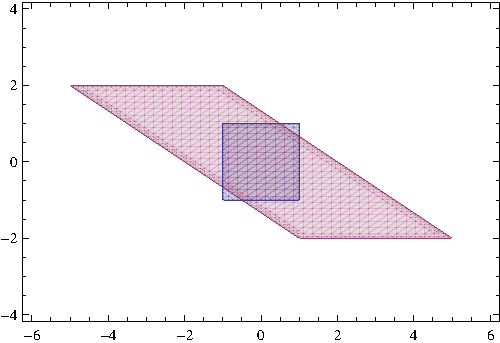
\includegraphics[width=\columnwidth]{infty.pdf}%
	\end{figure}
	\end{column}
	\end{columns}
	\begin{block}{В общем случае}
	$$
	\|\A\|_\infty = \max_i \sum_j |a_{ij}|
	$$
	\end{block}
\end{frame}

\begin{frame}
	\frametitle{Матричная норма $\|\cdot\|_\one$}
	\begin{columns}[T]
	\begin{column}{0.6\textwidth}
	Точка
	$\x = \begin{psmallmatrix}
		0\\1
	\end{psmallmatrix}$
	 с нормой $\|\x\|_\one = 1$ переходит в точку $$\y = \A\x = \begin{pmatrix}
		-3\\2
	\end{pmatrix}$$
	 с нормой $\|\y\|_\one = 5$.

	Для остальных точек $\|\x\|_\one = 1$
	$$\|\A\x\|_\one \leqslant 5$$
	$$
	\|\A\|_\one = 5
	$$
	\end{column}

	\begin{column}{0.4\textwidth}
	$$
	\A = \begin{pmatrix}
		2&-3\\
		0&2
	\end{pmatrix}
	$$
	\begin{figure}%
	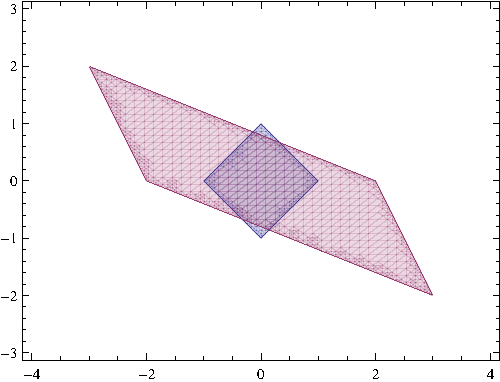
\includegraphics[width=\columnwidth]{l1.pdf}%
	\end{figure}
	\end{column}
	\end{columns}
	\begin{block}{В общем случае}
	$$
	\|\A\|_\one = \max_j \sum_i |a_{ij}| = \|\A^\tr\|_\infty
	$$
	\end{block}
\end{frame}

\begin{frame}
\frametitle{Матричная норма $\|\cdot\|_E$}
	\begin{columns}[T]
	\begin{column}{0.6\textwidth}
	Точка
	$\x = \frac{1}{\sqrt{5}}\begin{psmallmatrix}
		-1\\2
	\end{psmallmatrix}$
	 с нормой $\|\x\|_E = 1$ переходит в точку $$\y = \A\x = \frac{1}{\sqrt{5}}\begin{pmatrix}
		-8\\4
	\end{pmatrix}$$
	 с нормой $\|\y\|_E = 4$.

	Для остальных точек $\|\x\|_E = 1$
	$$\|\A\x\|_E \leqslant 4$$
	$$
	\|\A\|_E = 4
	$$
	\end{column}

	\begin{column}{0.4\textwidth}
	$$
	\A = \begin{pmatrix}
		2&-3\\
		0&2
	\end{pmatrix}
	$$
	\begin{figure}%
	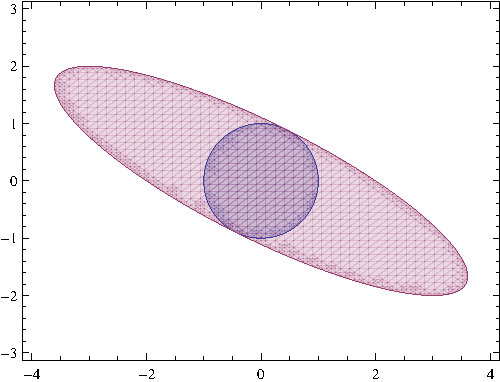
\includegraphics[width=\columnwidth]{euclid.pdf}%
	\end{figure}
	\end{column}
	\end{columns}
	\begin{block}{В общем случае}
	$$
	\|\A\|_E = \sigma_{\max}(\A) = \sqrt{\max \lambda(\A^\tr\A)}
	$$
	\end{block}
\end{frame}

\begin{frame}
\frametitle{Матричная норма $\|\cdot\|_E$}
	$$
	\A = \begin{pmatrix}
		2&-3\\
		0&2
	\end{pmatrix},\qquad
	\A^\tr\A = \begin{pmatrix}
		4&-6\\
		-6&13
	\end{pmatrix}
	$$
	Собственные числа матрицы $\A^\tr\A$: $\lambda_1 = 1, \lambda_2 = 16$, ортонормированные собственные вектора
	$$
	\x_1 = \frac{1}{\sqrt{5}}\begin{pmatrix}
		2\\1
	\end{pmatrix}, \quad
	\x_2 = \frac{1}{\sqrt{5}}\begin{pmatrix}
		-1\\2
	\end{pmatrix}, \quad
	$$
	$$
	\|\A\|_E = \sqrt{16} = 4
	$$
	Особенно просто норма $\|\cdot\|_E$ вычисляется в случае $\A = \A^\tr$
	$$
	\|\A\|_E = \sqrt{\max\lambda(\A^\tr\A)} = \sqrt{\max\lambda(\A^2)} = \max|\lambda(\A)|
	$$
\end{frame}

\section{Обусловленность}
\subsection{Фиксированная правая часть}
\begin{frame}
\frametitle{Число обусловленности системы}
	Рассмотрим систему
	$$
	\A\x = \b
	$$
	и <<близкую>> к ней систему
	$$
	\A(\x+\delta \x) = \b + \delta \b
	$$
	Оценим относительную погрешность решения
	$$
	\frac{\|\delta\x\|}{\|\x\|} \leqslant \frac{\|\A^{-1}\|\|\delta \b\|}{\|\x\|} =
	\frac{\|\A^{-1}\|\|\delta \b\|}{\|\A^{-1}\b\|} =
	\frac{\|\A^{-1}\|\|\b\|}{\|\A^{-1}\b\|}\frac{\|\delta \b\|}{\|\b\|}
	$$
	Обозначим $\nu(\A,\b) = \frac{\|\A^{-1}\|\|\b\|}{\|\A^{-1}\b\|}$
	\begin{block}{}
	$$\frac{\|\delta\x\|}{\|\x\|} \leqslant \nu(\A,\b) \frac{\|\delta \b\|}{\|\b\|}$$
	\end{block}
	Назовем $\nu(\A, \b)$ числом обусловленности системы $\A\x = \b$.
\end{frame}

\begin{frame}{Свойства числа обусловленности}
	\begin{block}{}
	$$\frac{\|\delta\x\|}{\|\x\|} \leqslant \nu(\A,\b) \frac{\|\delta \b\|}{\|\b\|}, \quad \nu(\A,\b) = \frac{\|\A^{-1}\|\|\b\|}{\|\A^{-1}\b\|}$$
	\end{block}
	Поскольку $\|\A^{-1}\b\| \leqslant \|\A^{-1}\|\|\b\|$
	$$
	\nu(\A,\b) \geq 1,
	$$
	причем существует такая правая часть $\b$, что $\nu(\A,\b) = 1$. Это именно то значение $\b$, при котором
	$$
	\| \A^{-1} \b \| = \|\A^{-1}\| \|\b\|
	$$
	При этом относительная погрешность решения не превосходит относительную погрешность правой части
\end{frame}

\subsection{Произвольная правая часть}
\begin{frame}
\frametitle{Произвольная правая часть}
	Посмотрим, насколько большой может быть величина $\nu(\A,\b)$ в зависимости от $\b$. С одной стороны,
	$$
	\nu(\A,\b) = \frac{\|\A^{-1}\|\|\b\|}{\|\A^{-1}\b\|} \geq 1
	$$
	Введем
	$$
	\mu(\A) = \max_{\b} \nu(\A, \b)
	$$
	$$
	\mu(\A) = \|\A^{-1}\|\max_{\b} \frac{\|\b\|}{\|\A^{-1}\b\|} = \|\A^{-1}\|\max_{\x} \frac{\|\A\x\|}{\|\x\|} = \|\A^{-1}\| \|\A\|
	$$
	Таким образом, для произвольной правой части
	\begin{block}{}
	$$\frac{\|\delta\x\|}{\|\x\|} \leqslant \mu(\A) \frac{\|\delta \b\|}{\|\b\|}, \quad \mu(\A) = \|\A\|\|\A^{-1}\|$$
	\end{block}
\end{frame}

\begin{frame}
\frametitle{Число обусловленности матрицы}
	Число $\mu(\A)$ называется обусловленностью матрицы $\A$ и показывает,
	насколько матрица <<близка>> к вырожденной. Поскольку
	$$
	\mu(\A) \geq \nu(\A,\b) \geq 1,
	$$
	относительная погрешность решения никогда не меньше относительной погрешности правой части. Более того, для любой матрицы $\A$
	можно найти такие $\b$ и $\delta \b$, что относительная погрешность решения будет ровно в $\mu(\A)$ раз больше относительной
	погрешности правой части.

	Эта погрешность связана с самой задачей решения СЛАУ, а не с конкретным методом ее решения, и ни один численный метод
	не может решить эту задачу точнее. Поэтому данная погрешность будет \emph{неустранимой}
\end{frame}

\begin{frame}[plain]
  \begin{center}
  {\Huge Спасибо за внимание!}
  \vspace{8ex}

  Цыбулин Иван

  e-mail: \colorhref{mailto:tsybulin@crec.mipt.ru}{tsybulin@crec.mipt.ru}
  \end{center}
\end{frame}

\end{document}
